\section{Results}\label{sec:results}

\subsection{Measurement protocol}\label{sec:measure}

For each ``system $\times$ strategy'' pair, we performed $R$ independent runs with fixed generator seeds: $R=100$ for levels A and B, the synthetic families, and the ablation; $R=50$ for the hyperparameter, horizon, bisection, and enlarged-region tests; and $R=10$--$100$ for the coupled systems. A run stopped at the first hit of the target or when the budget was exhausted. Common random numbers were used: the first 50 points of all strategies coincide with the first 50 points of uniform sampling, so differences arise only after the initial sample. $N_{0.9}$ is the 0.9 quantile of the first-hit time (infinity if fewer than 90\% of the runs find the target). Confidence intervals are 95\% bootstrap intervals over runs\cite{EfronTibshirani1994} (2000 resamples). The exponent $s$ is the slope of the regression of $\ln N_{0.9}$ on $\ln(1/p)$. Uniform sampling for the coupled systems and the enlarged regions was run on a GPU with a kernel that reproduces the CPU trajectories and fingerprints bit for bit. Unless stated otherwise, gains refer to the number of integrations with full integration. In the cost measurements (Sec.~\ref{sec:cost}), we also record integrator steps (a step of the observation window counts twice, because the companion trajectory for the Lyapunov exponent is integrated alongside) and wall time, measured after an untimed warm-up that compiles the kernels; steps and time up to the first hit are counted in proportion to the position of the hit within its batch. We compare uniform sampling, Zelinka's DE, splitting by $\xi$ from Eq.~\eqref{eq:xi}, active learning with 20\% uniform points, the portfolio, and the portfolio with nullclines (channel C). The final configuration of the portfolio (Sec.~\ref{sec:cost}) adds two-stage evaluation and the capped boundary arm; on runs shorter than $2\times10^4$ evaluations, the cap changes nothing. The library and the experiment scripts were written with the assistance of the AI coding assistant Claude (Anthropic; used through Claude Code in 2026, most recent model Claude Fable 5.1) to speed up the implementation of the author's specifications; all numerical results were produced by this code from fixed seeds, and the code was verified by the bit-exactness tests between the CPU and GPU kernels, by the independent integrators of Sec.~\ref{sec:protocol}, and by the agreement of its labels with Attractors.jl (Sec.~\ref{sec:cost}).

\subsection{Rare targets of levels A and B}\label{sec:rare_ab}

The results are summarized in Table~\ref{tab:gains} and Fig.~\ref{fig:pn}. The portfolio outperforms uniform sampling with statistical significance (the lower bound of the interval exceeds 1) on Chua~II (7.4 times), SE11 (3.1), and LE1 (6.2); with nullcline sampling, it also gains on Chua~I (4.4 times). On LE1, the best single arm is splitting (8.3 times), whereas active learning loses to uniform sampling (0.48): the long ``continuum of equilibria/escape'' boundary attracts the queries, and the target adjoins it only along a small part. The portfolio limits this degradation. On three problems, the portfolio gains little or nothing: the Jafari cycle, the Jafari chaos, and the Huynh map. These are predicted failures (Sec.~\ref{sec:failures}), and the portfolio stays within the guarantee of Proposition~\ref{prop:portfolio} ($G\ge\varepsilon=0.2$): 0.43, 0.42, and 1.40. Zelinka's DE, which is told the size of the target, is nowhere significantly better than uniform sampling; on the Jafari chaos and cycle, it loses by factors of 4.3 and 3.4. On the Jiang maps ($p\approx0.03$--$0.07$), all strategies are close to uniform sampling: at such $p$, the target is often found within the initial sample, and adaptation has nothing to work with. The contributions of the arms (ablation), the comparison with bisection toward basin boundaries, and the robustness to hyperparameters and to the integration horizon are given in Appendix~\ref{app:ablation}; no hyperparameter variant brings the gain below 1, and scaling both integration windows by 0.5 or 2 keeps the gains within 20\% of the base values.

\begin{table*}
\caption{Gain factors $G_{0.9}=N^0_{0.9}/N_{0.9}$ with 95\% bootstrap intervals ($R=100$). Bold: values whose lower interval bound exceeds 1.}
\label{tab:gains}
\footnotesize
\setlength{\tabcolsep}{4pt}
\begin{ruledtabular}
\begin{tabular}{lrrrrrrr}
System & $p$ & $N^0_{0.9}$ & \shortstack{Zelinka's\\DE} & Splitting & \shortstack{Active learning\\+ 20\% uniform} & Portfolio & \shortstack{Portfolio\\+ nullclines} \\
\hline
Chua I & 0.035 & 66 & 0.60 \ci{0.43}{0.99} & 1.20 \ci{0.92}{1.77} & 1.23 \ci{0.95}{1.74} & 1.24 \ci{0.94}{1.77} & \textbf{4.42} \ci{3.27}{6.47} \\
Chua II & 0.0027 & 818 & 0.84 \ci{0.67}{1.32} & \textbf{5.05} \ci{4.13}{7.07} & \textbf{3.16} \ci{2.58}{4.90} & \textbf{7.36} \ci{6.09}{10.2} & \textbf{7.64} \ci{5.98}{11.8} \\
SE11 & 0.0079 & 317 & 0.95 \ci{0.72}{1.07} & \textbf{2.53} \ci{1.95}{2.86} & \textbf{3.62} \ci{2.63}{4.16} & \textbf{3.10} \ci{2.46}{3.70} & \textbf{3.56} \ci{2.71}{4.31} \\
LE1 & 0.0016 & 1617 & 1.31 \ci{0.94}{2.08} & \textbf{8.29} \ci{6.35}{12.3} & 0.48 \ci{0.32}{1.49} & \textbf{6.24} \ci{3.76}{10.0} & \textbf{4.62} \ci{3.03}{10.7} \\
Jafari 2026, cycle & 0.009 & 219 & 0.29 \ci{0.19}{0.50} & 0.29 \ci{0.19}{0.53} & 0.88 \ci{0.66}{1.41} & 0.43 \ci{0.29}{0.78} & 0.32 \ci{0.25}{0.50} \\
Huynh 2019 & 0.0091 & 221 & 0.45 \ci{0.34}{0.85} & 1.36 \ci{0.79}{2.42} & 0.82 \ci{0.57}{1.72} & \textbf{1.40} \ci{1.16}{2.54} & --- \\
Jafari 2026, chaos & $(2$--$4)\times10^{-4}$ & 5265 & 0.23 \ci{0.16}{0.28} & 0.22 \ci{0.15}{0.28} & 1.08 \ci{0.57}{1.40} & 0.42 \ci{0.29}{0.58} & 0.27 \ci{0.16}{0.32} \\
\hline
Jiang NF I e/f/g & 0.028--0.039 & 109/86/71 & 0.83/0.90/1.00 & 1.52/1.23/1.08 & 1.02/1.51/1.15 & 1.46/1.49/1.23 & --- \\
Jiang SF I a/b & 0.065 & 36/33 & 0.75/0.92 & 1.00/1.00 & 1.00/1.00 & 1.00/1.00 & --- \\
\end{tabular}
\end{ruledtabular}
\end{table*}

\begin{figure*}
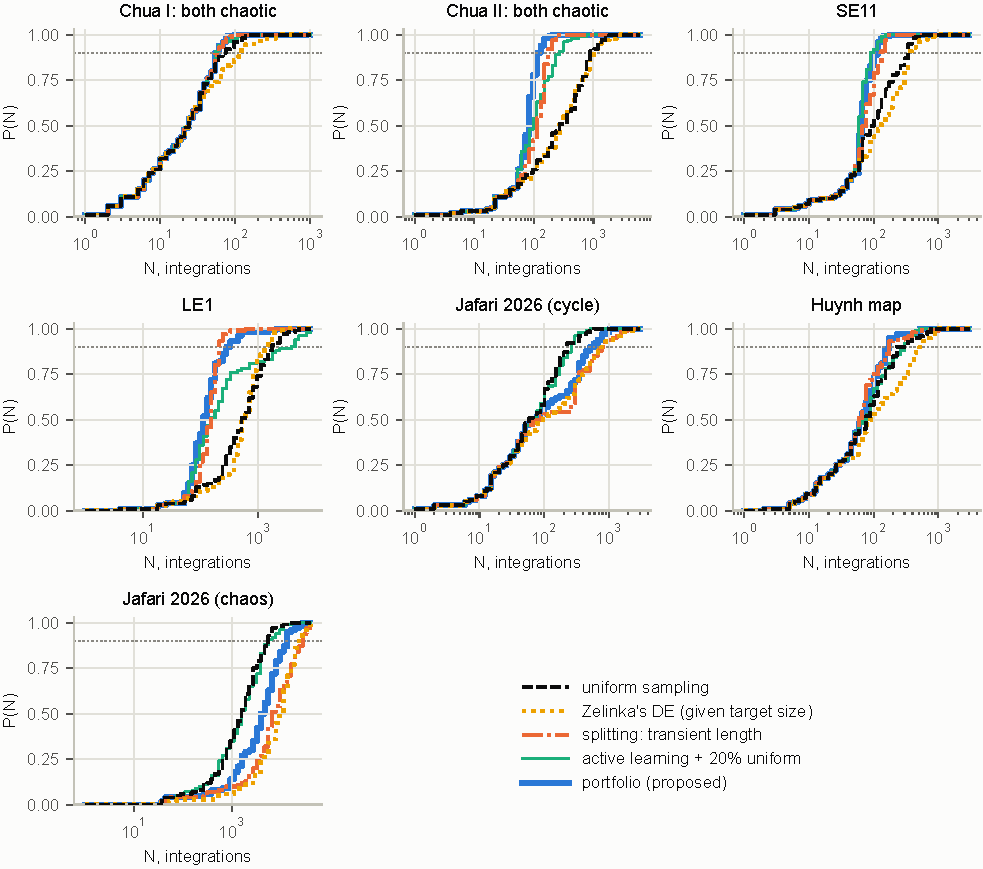
\includegraphics[width=\textwidth]{figures/fig21_pn_levelAB.pdf}
\caption{Detection probability $P(N)$ as a function of the number of integrations for rare targets of levels A and B ($R=100$ runs). The dotted line is the 0.9 level. On Chua~II, SE11, and LE1, the portfolio curve (thick blue) lies to the left of uniform sampling (gray) over the whole range; on the Jafari cycle and chaos, it lies to the right, but within the guaranteed factor $1/\varepsilon$.}
\label{fig:pn}
\end{figure*}

\subsection{Scaling with basin measure and dimension}\label{sec:scaling_p}

On family D2 ($n=6$), the gain grows as $p$ decreases from $10^{-2}$ to $10^{-5}$ (Table~\ref{tab:scaling}, Fig.~\ref{fig:scalp}). The scaling exponent of the portfolio is $s=0.45$ [0.42, 0.51], and that of splitting by $\xi$ is $0.41$ [0.37, 0.46], against $0.99$ [0.93, 1.04] for active learning and $0.95$ [0.90, 1.03] for uniform sampling (theoretical value 1). On a problem with a graded signal, the method thus gains in order: at $p=10^{-5}$, the gain is 93-fold for splitting and 72-fold for the portfolio. On family D1, where there is no signal outside the thin rim of the ball, all strategies have $s$ from 0.67 to 0.98; splitting does not help ($G=0.49$--$0.70$), and active learning gives a factor of 1.1--3.5 that grows as $p$ decreases, because escapes inside the ball serve as boundary markers. This is the prediction of Proposition~\ref{prop:cost} for a coordinate with zero informative depth.

Below $p=10^{-5}$, the gain on D2 breaks down: at $p=10^{-6}$, within $2\times10^5$ integrations, the portfolio finds the target in 35\% of runs against 18\% for uniform sampling, and at $10^{-7}$, within $10^6$ integrations, in 16\% against 9.5\%. The breakdown is the discretization limit of Sec.~\ref{sec:costmodel}: the coordinate is informative only in the zone $|w_0|\lesssim\rho/\sqrt{2\kappa\Delta t}$, which occupies 2.3\% of the region at $p=10^{-5}$, 0.23\% at $10^{-6}$, and 0.023\% at $10^{-7}$, so an initial sample of 50 points contains an informative point with probability 0.68, 0.11, and 0.011. Reducing the integration step restores the gain: fourfold at $p=10^{-6}$ gives $G=450$ for the portfolio and 530 for splitting, and sixteenfold at $p=10^{-7}$ gives 1200 and 1400, with all runs successful (Appendix~\ref{app:smallp}). The limit is set by the time resolution of the reaction coordinate rather than by splitting. The same limit explains the dependence on dimension at fixed $p=10^{-4}$ (Appendix~\ref{app:smallp}): the portfolio gains 17 times at $n=6$, 42 at $n=8$, 53 at $n=10$, 61 at $n=12$, and 45 at $n=14$, but nothing at $n=4$, where the basin in the additional coordinate has width $\rho=6.6\times10^{-4}$ and the coordinate is flat on 99.5\% of the region.

\begin{table}
\caption{Family D2 ($n=6$): cost of uniform sampling $N^0_{0.9}$ (in parentheses, the theoretical value $\ln10/p$) and the costs and gains of splitting and of the portfolio ($R=100$). For $p\le10^{-6}$, the budget of the strategies ($2\times10^5$ at $p=10^{-6}$ and $10^6$ at $p=10^{-7}$) is smaller than $N^0_{0.9}$, and the fraction of runs that found the target within it is given, with that of uniform sampling in brackets.}
\label{tab:scaling}
\begin{ruledtabular}
\begin{tabular}{rrrr}
$p$ & Uniform & Splitting & Portfolio \\
\hline
$10^{-2}$ & 277 (230) & 121 (2.3$\times$) & 122 (2.3$\times$) \\
$10^{-3}$ & 1932 (2303) & 262 (7.4$\times$) & 329 (5.9$\times$) \\
$10^{-4}$ & 17\,416 (23\,026) & 714 (24$\times$) & 1026 (17$\times$) \\
$10^{-5}$ & 189\,765 (230\,259) & 2039 (93$\times$) & 2634 (72$\times$) \\
$10^{-6}$ & $2.19\times10^{6}$ ($2.30\times10^{6}$) & 24\% [18\%] & 35\% [18\%] \\
$10^{-7}$ & $2.14\times10^{7}$ ($2.30\times10^{7}$) & 9\% [9.5\%] & 16\% [9.5\%] \\
\end{tabular}
\end{ruledtabular}
\end{table}

\begin{figure*}
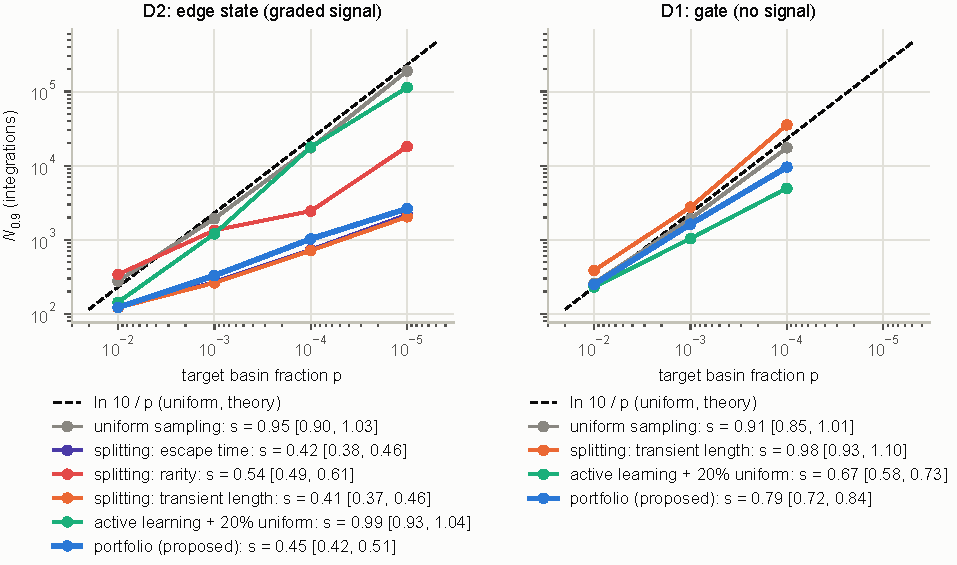
\includegraphics[width=\textwidth]{figures/fig23_scaling_p.pdf}
\caption{Detection cost $N_{0.9}$ versus basin measure $p$ ($n=6$, $R=100$); the legends give the scaling exponents $s$, defined by $N_{0.9}\propto p^{-s}$, with 95\% intervals. Left: family D2 with a graded signal; the splitting arms and the portfolio have $s\approx0.4$--$0.45$. Right: family D1 without a signal; all strategies have $s\approx0.7$--$1$. Dashed line: $\ln10/p$.}
\label{fig:scalp}
\end{figure*}

\subsection{Coupled systems: rare hidden targets and a new attractor}\label{sec:coupled}

\textbf{Coupled copies of SE11.} A real system with a rare hidden target is obtained by coupling several copies of a system with a hidden attractor. We take $k$ copies of SE11 with mean-field coupling along $y$:
\begin{equation}
\dot{\bm x}_u=\bm F(\bm x_u)+\epsilon\,\bigl(\bar y-y_u\bigr)\,\bm e_y,\qquad u=1,\dots,k,
\label{eq:coupled}
\end{equation}
where $\bar y=k^{-1}\sum_{v}y_v$ and $\epsilon=0.01$, in the region $B^k$. The only equilibrium is the synchronous equilibrium of SE11, which is stable, so the regime ``all copies on the hidden attractor'' is hidden. Its basin measure is $5.5\times10^{-5}$ for $k=2$ ($n=6$) and $3.5\times10^{-7}$ for $k=3$ ($n=9$), close to $p_1^k$ for independent copies ($p_1=0.0079$). Here the portfolio gains by orders of magnitude (Table~\ref{tab:coupled}): 65 \ci{42}{87} at $n=6$ and 1400 \ci{900}{2400} at $n=9$, where it needs about $5\times10^3$ integrations instead of $7.6\times10^6$; all runs found the target. The transient duration is set by the copies that have not yet settled, so successive levels of splitting fix the copies one after another, and the cost grows roughly geometrically in $k$ with a ratio far smaller than $1/p_1$. Without coupling, the gains are the same (1600 at $n=9$), and with four uncoupled copies ($n=12$, $p=p_1^4=3.9\times10^{-9}$), the portfolio finds the target in $N_{0.9}=4.7\times10^4$ integrations, a gain of $1.3\times10^4$ relative to the exact uniform cost $\ln10/p$. Bisection toward basin boundaries does not scale on these systems: within budgets of $8/p$ at $n=6$ and $2\times10^5$ at $n=9$, it finds the target in 66\% and 32\% of runs. The coupling is weak, and the problem is close to a product of independent ones; if the attractors of a single copy are known, product initial conditions reach such a target directly, so the coupled copies test the mechanism of the gain rather than replace that shortcut.

\begin{table*}
\caption{Coupled copies of SE11, Eq.~\eqref{eq:coupled}: basin measure of the regime ``all copies on the hidden attractor,'' cost of uniform sampling, and gains $G_{0.9}$ with 95\% bootstrap intervals ($R=100$ for $n=3$ and for $n=9$ with coupling; $R=50$ otherwise). For $n=12$, $N^0_{0.9}=\ln10/p_1^4$ is the exact geometric value. Bold: values whose lower interval bound exceeds 1.}
\label{tab:coupled}
\footnotesize
\setlength{\tabcolsep}{3pt}
\begin{ruledtabular}
\begin{tabular}{rrrrrr}
$n$ & $\epsilon$ & $p$ & $N^0_{0.9}$ & Splitting & Portfolio \\
\hline
3 & --- & $7.7\times10^{-3}$ & 317 & \textbf{2.53} \ci{1.95}{2.86} & \textbf{3.10} \ci{2.46}{3.70} \\
6 & 0.01 & $5.5\times10^{-5}$ & $3.8\times10^{4}$ & \textbf{44.0} \ci{27.0}{65.6} & \textbf{64.9} \ci{41.7}{86.6} \\
9 & 0.01 & $3.5\times10^{-7}$ & $7.6\times10^{6}$ & \textbf{682} \ci{448}{989} & \textbf{1435} \ci{896}{2372} \\
9 & 0 & $4.9\times10^{-7}$ & $5.3\times10^{6}$ & \textbf{598} \ci{325}{1000} & \textbf{1574} \ci{771}{2299} \\
12 & 0 & $3.9\times10^{-9}$ & $5.9\times10^{8}$ & \textbf{4881} \ci{3860}{6354} & \textbf{12\,681} \ci{9827}{18\,098} \\
\end{tabular}
\end{ruledtabular}
\end{table*}

\textbf{Two coupled Chua circuits.} The trajectories of SE11 mostly escape, so a uniform sample is cheap (Sec.~\ref{sec:cost}). A system in which all trajectories are bounded is obtained from two Chua~II circuits with mutual coupling $\epsilon(\bar x-x_u)$ in the first equation, $\epsilon=0.1$. The nine equilibria (products of the equilibria of the single circuit) are found by Newton's method; the regimes of the coupled system are enumerated by the identification protocol on a uniform sample of $5\times10^4$ points, with the products of the attractors and stable equilibria of the single circuit as initial templates. The synchronized cycle LC takes 98\% of the region. The rare hidden family consists of the regimes in which one circuit is on a hidden chaotic attractor and the other is at a stable equilibrium (and, at weaker coupling, both on hidden attractors); its total basin measure is $2.3\times10^{-5}$, and no trajectory from the $10^{-3}L$ and $10^{-2}L$ neighborhoods of the equilibria reaches it. On this target, with two-stage evaluation, the portfolio needs $N_{0.9}=1900$ integrations against $1.05\times10^5$ for uniform sampling ($R=20$, all runs successful), a gain of 55 in integrations and 64 in wall time (Table~\ref{tab:cost}). Three uncoupled copies of Chua~II give the extreme case: the regime ``every copy on one of its two hidden attractors'' has $p=(p_a+p_b)^3=1.9\times10^{-8}$ exactly, beyond uniform sampling ($\ln10/p=1.2\times10^8$ integrations, about four days of computing); the final configuration of the portfolio finds it in 9 of 10 runs within $4\times10^5$ integrations, with a median of $8.6\times10^4$ and $N_{0.9}=3.2\times10^5$, a gain of 370 in integrations and 150 in time.

\textbf{A hidden attractor born by the coupling.} The same enumeration revealed a regime that the single circuit does not have (Fig.~\ref{fig:newattr}): one circuit stays on the large cycle LC, and the other hops chaotically between the regions of the two hidden attractors HA$_a$ and HA$_b$, which in the single circuit at these parameters never merge.\cite{Stankevich2017} The regime passes the verification protocol (lifetime over $2\times10^3$ time units, the same template at $dt/2$, $\lambda=0.10$), and it is hidden: none of 3624 trajectories started in the $10^{-3}L$ and $10^{-2}L$ neighborhoods of the nine equilibria and along their unstable directions reaches it ($h_\varepsilon=0.18$ at $10^{-1}L$, as for Chua~I). Continuation in the coupling shows how it arises: for $\epsilon<0.045$, the second circuit oscillates periodically near one of its stable equilibria (four symmetric periodic regimes); at $\epsilon\approx0.045$, these branches merge into the chaotic hopping; $\lambda$ grows almost linearly to 0.35 at $\epsilon=0.46$, with periodic windows at $\epsilon=0.09$ and $0.47$; and at $\epsilon\approx0.5$, the two branches merge with the synchronized cycle. Coupled Chua circuits with hidden attractors have been studied for synchronization,\cite{Stankevich2017,Kuznetsov2023Chua} and we have not found this regime reported. It is hidden but not rare: its basin fraction is 0.6--1\% per symmetric branch at all $\epsilon$. Table~\ref{tab:newattr} compares how fast the search methods find it: the standard procedure never does, uniform sampling and the portfolio find it within a few hundred integrations, and if the attractors of the single circuit are known, the product initial condition ``LC $\times$ HA$_a$'' lands on it in one integration, because the regime continues that product state. The value of the method here is the enumeration with verification rather than speed.

\begin{figure*}
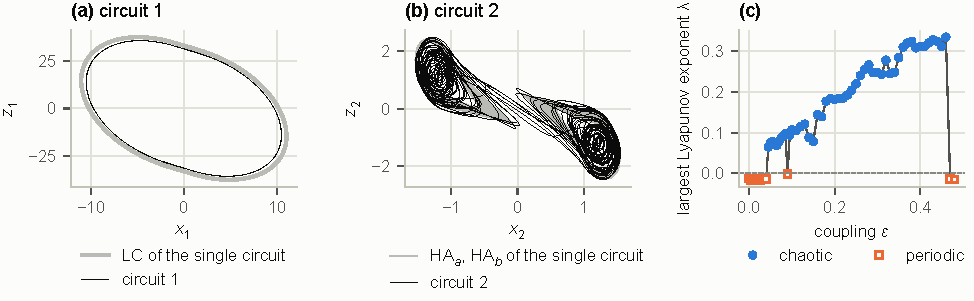
\includegraphics[width=\textwidth]{figures/fig31_new_attractor.pdf}
\caption{Hidden attractor of two coupled Chua~II circuits born by the coupling ($\epsilon=0.1$). (a) Circuit 1 in the projection $(x_1,z_1)$ against the cycle LC of the single circuit. (b) Circuit 2 in $(x_2,z_2)$ against the hidden attractors HA$_a$ and HA$_b$ of the single circuit (gray): the trajectory hops between their regions. (c) Largest Lyapunov exponent of the regime versus the coupling, from continuation in $\epsilon$: chaos is born at $\epsilon\approx0.045$ by merging of periodic branches and disappears at $\epsilon\approx0.5$.}
\label{fig:newattr}
\end{figure*}

\begin{table}
\caption{Finding the coupling-born attractor of Fig.~\ref{fig:newattr} (basin fraction 0.016 for the two symmetric branches): integrations to detection (0.9 quantile and median over $R=20$ runs) and wall time $T_{0.9}$ on one thread. The times of uniform sampling with two-stage evaluation and of the portfolio are measured; those of full integration and of recurrence-based stopping (Attractors.jl, Sec.~\ref{sec:cost}) are rescaled from the two-stage time by the measured ratio of costs per evaluation.}
\label{tab:newattr}
\footnotesize
\begin{ruledtabular}
\begin{tabular}{lrrr}
Method & $N_{0.9}$ & Median & $T_{0.9}$, s \\
\hline
From neighborhoods of the equilibria & never & --- & --- \\
Uniform sampling, full integration & 230 & 18 & 28 \\
Uniform sampling, two-stage evaluation & 230 & 18 & 17 \\
Uniform sampling, Attractors.jl & 230 & 18 & 6.4 \\
Portfolio (final configuration) & 81 & 18 & 8.1 \\
Product of single-circuit attractors & 1 & 1 & 0.07 \\
\end{tabular}
\end{ruledtabular}
\end{table}

\subsection{Cost in integrator steps and wall time}\label{sec:cost}

The number of integrations is a fair measure of cost only if all integrations cost about the same. They do not when trajectories escape: an escaping trajectory stops at the step of escape, and the method deliberately concentrates on long-lived trajectories. We therefore measured the cost of the final configuration in integrator steps and wall time (Table~\ref{tab:cost}, Fig.~\ref{fig:cost}). The final configuration is the three-arm portfolio with two-stage evaluation (Sec.~\ref{sec:twostage}), brute-force neighbor search, and the boundary arm trained on the last $2\times10^4$ points; for coupled systems, all products of the attractors of single units except the target are declared known. The reference is uniform sampling with the same two-stage evaluation. The gains are $G_N$ in integrations, $G_S$ in steps, and $G_T$ in time ($R=20$; three copies of Chua~II: $R=10$).

\begin{table*}
\caption{Cost of the final configuration of the portfolio relative to uniform sampling, both with two-stage evaluation ($R=20$; three copies of Chua~II: $R=10$, 9 successful runs): mean integrator steps per evaluation and gains in integrations ($G_N$), steps ($G_S$), and wall time ($G_T$, four threads per process). Bold: $G_T>1$. For uncoupled copies of Chua~II, uniform sampling is out of reach, and its cost is $\ln10/p$ evaluations at the measured cost per evaluation.}
\label{tab:cost}
\footnotesize
\begin{ruledtabular}
\begin{tabular}{lrrrrrrr}
Problem & $n$ & $p$ & \multicolumn{2}{c}{Steps per evaluation} & $G_N$ & $G_S$ & $G_T$ \\
 & & & Uniform & Portfolio & & & \\
\hline
%TABCOST-BEGIN
Chua I & 3 & $3.3\times10^{-2}$ & $2.6\times10^{4}$ & $4.6\times10^{4}$ & 1.0 & 0.27 & 0.25 \\
SE11 & 3 & $7.7\times10^{-3}$ & 1139 & 3681 & 4.1 & 0.92 & 0.84 \\
LE1 & 3 & $1.3\times10^{-3}$ & 334 & $1.1\times10^{4}$ & 2.1 & 0.052 & 0.085 \\
D2, $p=10^{-4}$ & 6 & $1.0\times10^{-4}$ & 14 & 1169 & 12 & 0.078 & 0.12 \\
D2, $p=10^{-5}$ & 6 & $1.0\times10^{-5}$ & 2 & 616 & 120 & 0.32 & \textbf{1.6} \\
2 coupled SE11 & 6 & $5.5\times10^{-5}$ & 117 & 3694 & 49 & 1.2 & \textbf{1.0} \\
3 coupled SE11 & 9 & $3.5\times10^{-7}$ & 45 & 3418 & 2600 & 30 & \textbf{22} \\
Chua II & 3 & $2.6\times10^{-3}$ & $8.7\times10^{4}$ & $9.7\times10^{4}$ & 6.3 & 5.3 & \textbf{3.8} \\
2 Chua II, $\epsilon=0.1$ & 6 & $2.3\times10^{-5}$ & $3.0\times10^{5}$ & $3.4\times10^{5}$ & 55 & 49 & \textbf{64} \\
2 Chua II, $\epsilon=0$ & 6 & $7.2\times10^{-6}$ & $1.7\times10^{5}$ & $1.9\times10^{5}$ & 200 & 160 & \textbf{130} \\
3 Chua II, $\epsilon=0$ & 9 & $1.9\times10^{-8}$ & $1.7\times10^{5}$ & $2.3\times10^{5}$ & 370 & 270 & \textbf{150} \\
%TABCOST-END
\end{tabular}
\end{ruledtabular}
\end{table*}

\begin{figure}
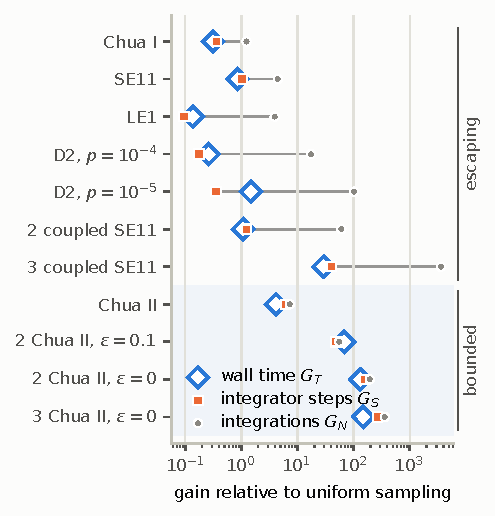
\includegraphics[width=\columnwidth]{figures/fig30_cost_gains.pdf}
\caption{Gain of the portfolio relative to uniform sampling in integrations ($G_N$), integrator steps ($G_S$), and wall time ($G_T$), both with two-stage evaluation. Above the dotted line: systems in which most trajectories escape quickly; below: systems with bounded trajectories. Dashed line: $G=1$.}
\label{fig:cost}
\end{figure}

The problems fall into two groups. In the systems where most trajectories escape quickly (Chua~I, SE11, LE1, D2, coupled SE11), the portfolio spends 2--300 times more steps per evaluation than uniform sampling, because it selects exactly the long transients that lead toward the target, whereas most uniform points escape within a few steps. The gain in integrations then shrinks in steps by a factor of 4--400, and the portfolio is slower than uniform sampling in time on Chua~I, SE11, LE1, and D2 at $p=10^{-4}$ (0.085--0.84). It gains in time only where the gain in integrations is large: 1.6 on D2 at $p=10^{-5}$ ($G_N=120$) and 22 on three coupled copies of SE11 ($G_N=2600$). In the systems with bounded trajectories (Chua~II and its coupled and uncoupled copies), every trajectory runs over the full horizon unless the two-stage evaluation stops it, the steps per evaluation of the portfolio and of uniform sampling are close, and the gain carries over to time: 3.8 on Chua~II, 64 on the coupled circuits, and 130--150 on the uncoupled copies. Two-stage evaluation makes both methods faster, uniform sampling more so: on Chua~II, 94\% of the uniform points and 91\% of the points of the portfolio stop at stage~1. Product references matter for coupled systems: they let stage~1 stop the trajectories that settle onto mixed states and give the boundary arm informative classes instead of ``unknown''; on three coupled copies of SE11, $N_{0.9}$ falls from 3500 to 2100 and $G_T$ grows from 4 to 12. The own computations of the arms take 1--8\% of the time on the Chua systems and 20--60\% on the cheap problems, mostly the nearest-neighbor queries of the boundary arm; brute-force search for $n\ge6$ reduces them by a factor of 1.6--2.6 ($G_T$ from 12 to 22 on three coupled copies of SE11), and the cap on the training sample removes their growth in long runs: on three uncoupled copies of Chua~II, it lowers the overhead from 51\% to 28\% and, by training the classifier on recent points only, also lowers the median cost from $1.4\times10^5$ to $8.6\times10^4$ integrations, so $G_T$ grows from 64 to 150. A wider batch, with two or four times more chains and boundary points to occupy more cores, does not pay: the number of evaluations grows by a factor of 1.5--3, whereas the time per evaluation decreases by about 10\% only.

\textbf{Comparison with recurrence-based evaluation.} The cost of one evaluation can be reduced further by stopping a trajectory as soon as it recurs in the cells of an already known attractor, as in Attractors.jl.\cite{DatserisWagemakers2022,Datseris2023Framework} For uniform sampling, the index of the first point in the target basin does not depend on how the trajectories are evaluated, so the time of uniform sampling with any evaluation scheme is $N^0_{0.9}$ times the mean cost of one evaluation, and the schemes can be compared on a common set of initial conditions. Table~\ref{tab:time} compares, on one thread, full integration, our two-stage evaluation, and \textsc{AttractorsViaRecurrences} (Attractors.jl 2.0, sparse grid of 100 cells per dimension, sampling interval 0.1, adaptive Tsit5 with tolerance $10^{-9}$ or fixed-step RK4 with our step), whose labels on the first 500 points coincide with ours and which recognizes the target states fed to it. On the bounded Chua systems with long transients, recurrence-based stopping is 2--3 times cheaper per evaluation than our two-stage evaluation, which still needs the early window and a quarter of the observation window for the fingerprint; on the escaping systems, our evaluation is 2--8 times cheaper, because escape is detected by the radius at once. Against uniform sampling with recurrence-based stopping, the time gain of the portfolio on the coupled Chua circuits falls from 27 to 10, and on Chua~II from 5 to 1.6; the gain in integrations is untouched. The search strategy and the evaluation back-end are independent choices: the portfolio needs only a regime label and a transient duration for each point, both of which the recurrence mapper provides, so combining the two would return the time gain to the gain in integrations.

\begin{table*}
\caption{Uniform sampling with three evaluation schemes against the portfolio, on one thread ($R=20$): cost of one evaluation (ms), time to detection $T_{0.9}$ (s), and the time gain of the portfolio relative to uniform sampling with two-stage evaluation ($G_T$) and with recurrence-based stopping ($G_T^{\rm rec}$). For uniform sampling, $T_{0.9}=N^0_{0.9}$ times the cost of one evaluation; for the portfolio, the measured 0.9 quantile of the run time. Attractors.jl: the fastest of the tested settings (Tsit5). Bold: gains above 1.}
\label{tab:time}
\footnotesize
\setlength{\tabcolsep}{3pt}
\begin{ruledtabular}
\begin{tabular}{lrrrrrrrrrrrr}
Problem & $p$ & $N^0_{0.9}$ & \multicolumn{3}{c}{Cost per evaluation, ms} & \multicolumn{3}{c}{$T_{0.9}$ of uniform sampling, s} & \multicolumn{2}{c}{Portfolio} & $G_T$ & $G_T^{\rm rec}$ \\
 & & & full & two-stage & Attractors.jl & full & two-stage & Attractors.jl & $N_{0.9}$ & $T_{0.9}$, s & & \\
\hline
%TABTIME-BEGIN
Chua II & $2.6\times10^{-3}$ & 710 & 26.7 & 6.07 & 1.95 & 19 & 4.3 & 1.4 & 113 & 0.87 & \textbf{5.0} & \textbf{1.6} \\
2 Chua II, $\epsilon=0.1$ & $2.3\times10^{-5}$ & 104980 & 72.8 & 44.8 & 16.4 & 7.6e3 & 4.7e3 & 1.7e3 & 1899 & 172 & \textbf{27.3} & \textbf{10.0} \\
SE11 & $7.7\times10^{-3}$ & 294 & 0.131 & 0.0562 & 0.131 & 0.038 & 0.016 & 0.038 & 71 & 0.028 & 0.6 & \textbf{1.4} \\
LE1 & $1.3\times10^{-3}$ & 858 & 0.021 & 0.0108 & 0.0819 & 0.018 & 0.0093 & 0.07 & 413 & 0.58 & 0.016 & 0.12 \\
%TABTIME-END
\end{tabular}
\end{ruledtabular}
\end{table*}

\subsection{Failures and limits}\label{sec:failures}

All failures are kept in the paper: they delineate the domain of applicability of the method.
\begin{enumerate}
\item \textbf{Deceptive coordinate (Jafari 2026 chaos).} Almost all trajectories escape to infinity by slow drift, and the longest escapes lie in the region of slow drift rather than near the attractor. Splitting finds the target 4.5 times more slowly than uniform sampling ($G=0.22$); the portfolio stays within the guarantee (0.42).
\item \textbf{Deceptive transients in an enlarged region.} Enlarging the region of initial conditions $k$ times about its center does not make the hidden attractors of the benchmark rare: the basins extend far beyond the natural region, and $p$ falls by one or two orders of magnitude at most instead of $k^3$ (Appendix~\ref{app:enlarged}). On SE11, LE1, and Chua~I, the gain grows as $p$ falls (to 24, 16, and 6.3), but on Chua~II at $k=4$, the longest transients belong to trajectories returning from far away, splitting alone loses by a factor of 7, and the portfolio stays within the guarantee (0.71).
\item \textbf{Islands among escaping trajectories without a gradient of duration.} For the Jafari cycle, the escape time is determined by slow drift, and for the Huynh map, the escape times are discrete. No arm gains on the Jafari cycle, and the portfolio gains only 1.4 times on the Huynh map.
\item \textbf{Long boundaries of known basins to which the target adjoins along a small part (LE1).} The active-learning arm has a median 3.7 times better than uniform sampling but a heavy tail: 17 of 100 runs get stuck near a remote part of the boundary, and two do not find the target within the budget. In the portfolio, this tail is bounded (median 109, maximum 1859 evaluations).
\item \textbf{Discretization limit at very small $p$} (D2, $p\le10^{-6}$; Sec.~\ref{sec:scaling_p}).
\item \textbf{Cheap nontarget trajectories.} Where most trajectories escape within a few steps, a gain of 2--120 in integrations is a draw or a loss in time (Sec.~\ref{sec:cost}).
\item \textbf{First-generation strategies.} Adaptive splitting driven by asymptotic novelty finds the target on Chua~II in only 55\% of runs, and MAP-Elites with a behavior descriptor gives a median 4 times better than uniform sampling but a heavy tail, $G=0.39$. Such tails are precisely what the uniform share of the portfolio removes.
\end{enumerate}
The channel diagnostic $d(q)$ of Sec.~\ref{sec:costmodel}, measured on uniform samples, separates the cases of gain and failure on all seven problems where it was tested (Appendix~\ref{app:diagnostics}).
